\subsection{Opgaver}

\begin{enumerate}
	
	
	\item I denne opgave betragtes en kasse med højde $5cm$, længde $x$ og bredde $y$. Bestem det maksimale rumfang kassen kan have når bundens omkreds skal være $20cm$. 
	
	\item Find lokale maksimum og minimum for funktionen $f(x)=\frac{1}{4}x^4+\frac{1}{3}x^3-x^2+1$
	
	\item Et $ 300m $ langt hegn skal indhegne et rektangulært område. Bestem sidelængderne i rektanglet så arealet bliver størst muligt. 
	
	\item Brug differentialregning til at vise toppunktsformlen for et andengradspolynomium.
	
	\item En åben kasse skal have kvadratisk bund og et rumfang på $ 5000 cm^2 $. Bestem sidelængden i bunden og højden så kassens overfladeareal bliver mindst muligt.
	
	\item Funktionen $f$ givet ved $f(x)=ax^3+bx^2$ har et lokalt ekstremumspunkt i $(2,2)$. Bestem $a$ og $b$.
		
	\item \label{it:opt2exc} Et kvadrat og en ligebenet trekant er givet som i Figur~\ref{fig:opt2exc}.
	\begin{enumerate}
		\item Bestem $x$ så det samlede areal af kvadratet og trekanten bliver størst muligt.
		\item Bestem $x$ så det samlede areal af kvadratet og trekanten bliver mindst muligt.
	\end{enumerate}
	
		\begin{figure}
		\centering
		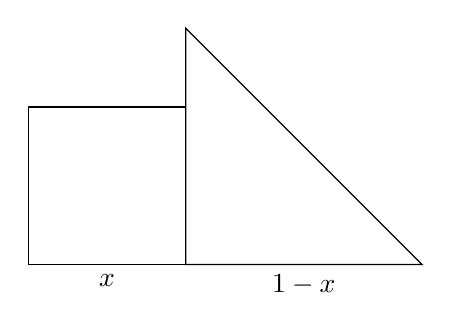
\begin{tikzpicture}
		\draw (0,0)--(0,2)--(2,2)--(2,0)--node[below] {$x$}cycle;
		\draw (2,0)--(2,3)--(5,0)--node[below] {$1-x$}cycle;
		\end{tikzpicture}
		\caption{Opgave~\ref{it:opt2exc}}
		\label{fig:opt2ëxc}
	\end{figure} 
	
	\item Har funktionen $f(x)=1-\sqrt[5]{x^2}$ et maksimum. Hvis ja så bestem det givne maksimum.
	

	
	\item Bestem de punkter hvor tangenthældningen til grafen for funktionen $f(x)=e^{-(x+1)^2}$ er størst og mindst. Hvad er den største og mindste tangenthældning. (Hint:	Bemærk at 
		\begin{align*}
		f''(x)=e^{-(x+1)^2}(4x^2+8x+2),
		\end{align*}
	samt at $e^{-(x+1)^2}>0$ for alle $x\in \R$.)


	\item Et rektangel er indskrevet i enhedscirklen som vist i \href{https://www.geogebra.org/m/efDNd8KK}{Geogebra} . Bestem sidelængderne så rektanglet får størst muligt areal. (Hint: Beskriv arealet af rektanglet ud fra punktet P.)
	
	\item En sekskant er indskrevet i enhedscirklen som vist i \href{https://www.geogebra.org/m/efDNd8KK}{Geogebra}. Bestem det størst mulige areal af sekskanten. (Hint: Beskriv arealet af sekskanten ud fra punktet P.)

	\item En trekant er indskrevet i enhedscirklen som vist i \href{https://www.geogebra.org/m/efDNd8KK}{Geogebra}. Bestem det størst mulige areal af trekanten. (Hint: Beskriv arealet af trekanten ud fra punktet P.)
	
	\item Et rektangel er placeret i et koordinatsystem således at det har et hjørnepunkt i origo, et på den positive del af $y$-aksen, et på den positive del af $x$-asksen. Det sidste hjørnepunkt er placeret på linjen $y=-3x+48$. Bestem sidelængderne på rektanglet som giver det størst mulige areal. Bestem også det maksimale areal af rektanglen.
	
	\item Et rektangel er placeret i et koordinatsystem således at det har et hjørnepunkt i origo, et på den positive del af $y$-aksen, et på den positive del af $x$-asksen. Det sidste hjørnepunkt er placeret på grafen for funktionen $\frac{\sin x}{x}$. Bestem sidelængderne på rektanglet som giver det størst mulige areal når $x\in[0\pi]$. Bestem også det maksimale areal af rektanglen.
	
	
	\item Lad $f(x)=x^2+4-4x$. I intervallet $]-2,2[ $ danner tangenten til $f$ samt $x$-aksen og $y$-aksen en retvinklet trekant. Bestem ligningen for den tangent der giver det størst mulige areal af trekanten. Bestem også arealet af denne trekant. Hvad er det mindst mulige areal areal af trekanten i det givne interval.
	
	\item\label{it:opt1} En kvadratisk plade med sidelængde $1$ skæres som vist Figur~\ref{fig:opt1} og foldes efterfølgende til en kasse uden top. Bestem $x$ så kassen rumfang bliver størst muligt.
	
	\item I denne opgave betragtes $3$ plader af typen som er afbildet i Figur~\ref{fig:opt1}. De afskårne kvadrater laves til to terninger. Bestem $x$ således de tre kasser uden låg og de to terninger får størst mulig fælles rumfang. 
	

	
	\begin{figure}
		\centering
		\begin{tikzpicture}
		\draw (0,0)--(0,5)--(5,5)--(5,0)--cycle;
		\draw[dashed] (1,0)--node[right] {$x$} (1,1)-- node[above] {$x$} (0,1);
		\draw[dashed] (4,0)--node[left] {$x$} (4,1)-- node[above] {$x$} (5,1);
		\draw[dashed] (5,4)--node[below] {$x$} (4,4)-- node[left] {$x$} (4,5);
		\draw[dashed] (0,4)--node[below] {$x$} (1,4)-- node[right] {$x$} (1,5);
		\draw[dotted] (1,1)--(4,1)--(4,4)--(1,4)--cycle;
		\end{tikzpicture}
		\caption{Opgave~\ref{it:opt1}}
		\label{fig:opt1}
	\end{figure} 


	\item Bestem den største og mindste værdi som funktionen $ g(x)=x^3+\frac{3}{4}x^2-\frac{3}{2}x $ antager intervallet
	\begin{enumerate}
		\item $ [-2,\frac{3}{2}] $,
		\item $ [-\frac{3}{2},1] $.
	\end{enumerate}
 
 	\item \label{it:opt3} I Figur~\ref{fig:opt3} ses en kegle med højde $H$ og radius $R$. Inden i denne kegle er en mindre kegle med højde $h$ og radius $r$ placeret på hovedet. Bestem $h$ og $r$ så rumfanget af den indre kegle bliver størst muligt. Bestem efterfølgende det maksimale rumfang af den lille kegle. (Hint: Rumfanget af en kegle med grundfladeareal $G$ og højde $h$ er $V=\frac{1}{3}Gh$. Brug at vinklen mellem grundfladen og siden af den store kegle er den samme som vinklen mellem grundfladen i den lille kegle og siden af den store kegle.)
 \begin{figure}
 	\centering
 	 \begin{tikzpicture}
 	\draw[dashed] (0,0) arc (170:10:2cm and 0.4cm)coordinate[pos=0] (a);
 	\draw (0,0) arc (-170:-10:2cm and 0.4cm)coordinate (b);
 	\draw[densely dashed] ([yshift=4cm]$(a)!0.5!(b)$) -- node[right,font=\footnotesize] {$H$} coordinate[pos=0.95] (c) ([yshift=2cm]$(a)!0.5!(b)$)-- node[right,font=\footnotesize] {$h$} coordinate[pos=0.95] (aa) ($(a)!0.5!(b)$)
 	-- node[above,font=\footnotesize] {$R$}coordinate[pos=0.05] (bb) (b);
	\draw (aa) -| (bb);
 	\draw (a) --node {} coordinate[pos=0.5] (aaa) ([yshift=4cm]$(a)!0.5!(b)$) -- node {} coordinate[pos=0.5](bbb) (b);
 	\draw[densely dashed] (aaa) arc (170:10:1cm and 0.2cm);
 	\draw (aaa) arc (-170:-10:1cm and 0.2cm);
 	\draw (aaa)--($(a)!0.5!(b)$)--(bbb);
 	\draw[densely dashed] ($(aaa)!0.5!(bbb) $)--node[above,font=\footnotesize] {$r$} coordinate[pos=0.1] (d) (bbb);
 	\draw (c)-| (d);
 	\end{tikzpicture}
 	\caption{Opgave~\ref{it:opt3}}
 	\label{fig:opt3}
 	
 	\item Vis Bernoullis ulighed,
 	\begin{align*}
 	(1+x)^r\geq 1+rx
 	\end{align*}
 	for $r\geq 1$ og $x>-1$. (Hint: Find minimum for funktionen $f(x)=(1+x)^r-(1+rx) $.)
 \end{figure}
\end{enumerate}